\chapter{Problem description}
%Give a label so yhat you can refer to this chapter:
\label{chap1}
{
Fist of all, We assume that the problems are foucs on the structured decentralization, of video on demand for peer-to-peer networks. We consider the network condition of the Internet is reliable or at least the bandwidth of each client is undiscrepant.There is no tracker server or media data center in the globle internet to mantian data.

In section 2.1 I will discuss the defects that bring up to centralized or semi-centralized P2P system which influents badly on the performance of VoD system based on the low-layer P2P network environment. But the transmission of bitstream of media resource mostly depends on these super nodes or clients. So it will affect the quality of Video-on-Demand such as delay or even out of service.

In section 2.2 the chanllenges of stream over decentralized peer-to-peer system is discussed based on the eminent P2P DHT algorithms currently. 
%The techniques of integration on video , audio and caption which makes up of the function of Video-on-Demand service will be explained in section 2.3.
}
\section{Decentaliation}
{
It was a great success of Peer-to-Peer techniques as the traffic of P2P applications have the weather gauge of the globle Internet in years before 2008, compared with the other protocols such as ftp, http, etc. 
The chart below illustrates the percent of P2P traffic ocupied compared with the other protocols.
\begin{center}
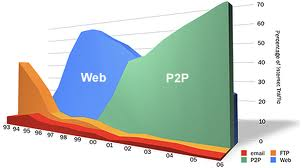
\includegraphics[width=5cm]{data/p2ptraffic.jpg}
\end{center}

However, New data from Arbor Networks shows that global P2P traffic is continuing to decline. 
Below there’s a graph posted by p2p-blog with the rate of decline, as compared with the overall Internet traffic between 2007 and 2009:
\begin{center}  
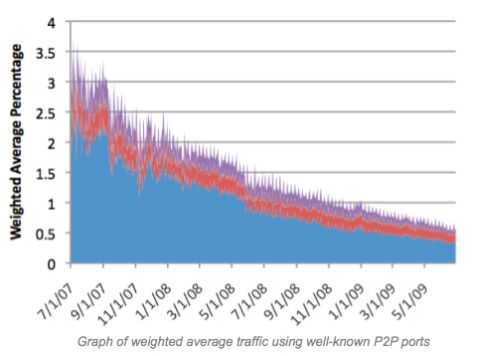
\includegraphics[width=5cm]{data/Arbor-Networks-graph-of-p2p-decline.jpg}
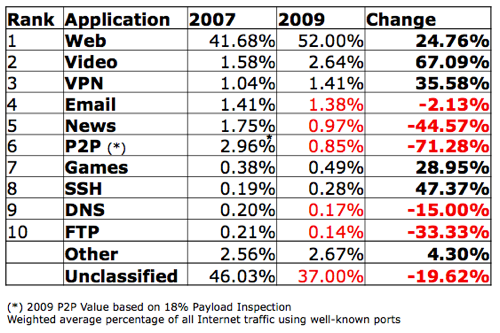
\includegraphics[width=5cm]{data/arbornetworks2-2.png}
\end{center}

There's a few interesting things to point out here: VPN traffic has been growing significantly at the same time as P2P traffic has been declining, which could at least in part be caused by P2P users signing up for VPN services to hide their activity.\cite{p2ptrafficdecline}

Obviously, this phenomemon indicates that on the suface P2P traffic declinies continusly and abundantly. On the other hand, the growing of VPN traffic enucleates that this kinds of shrink does not amount to vanish away but just migrate.
The root causes of this migratation is diversiform. 
However, we can deduce the most significant cause is the P2P applicaiton \emph{design objection} and \emph{vulnerable to attack}. 
So P2P users try to avoid these attacking and access blocked servers by using VPN, which seems to be an effective way to hide their actions. 
Unfortunately, most VPN services need extra fee to pay to these service providers before using it.
}

\subsection{Objections of Centralized P2P}
{
A typical Centralized P2P netorking is BitTorrent which implements multi-sources downloading and files distribution.
The basic fundamental of BitTorrent is the simultaneity of download and upload, which means when a user try to dowload resources from BT network, it also upload files or file segments to the others. So, the more users in the system , the faster will the files be downloaded. This incarnates the idea of 'tit-for-tat'.

When a user wants to share files or a directory, first of all, it has to generate a 'seed' file or 'metadata' file which contains the infomation about the shared files or directory and the URL of users.
And then upload the meta data to BT servers which are so called \emph{Tracker servers}.
Another user wants to download the shared file, it has to get to meta data from the Tracker servers, and then according to the infomation which is supported by the meta data to download the segments of shared files or directory from multipule resource nodes.
The follow chart illustrates the Architecture of BitTorrent:
\begin{center}
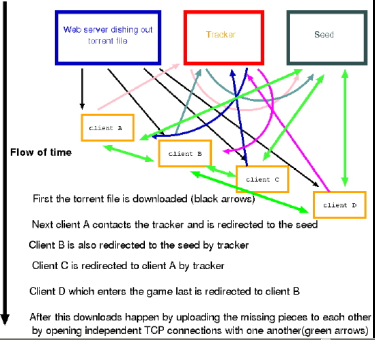
\includegraphics[width=8cm]{data/bittorrentprotocol.png}
\end{center}

From a structural point of view, BT belongs to centralized topology.
The Tracker servers are as a important part of the whole BT system, so the single point of failure performance failure should be inevitable. Moreover, BT does not support any search service, users have to login the BT published web server to find the files that he/she might be interested.

In this BT-liked centralized P2P networks, most noeds are connected with the centralized server or directory server which take the charge of indexing the context in all of the nodes. 
When request is sent, the centralized server will find all of the nodes which meet the qualifications of the request pre-sent. 
And then the file exchange will happen in the specified two nodes.

Taking one with another, the drawbacks of centralized P2P are as followed:
\begin{itemize}
\item Search calculation tasks are done by the centralized server, which may lead to a high requirements of server performance and bandwidth .
\item If the centralized server did not update in time, the result of the search task could not be accurate.
\item Due to the centralized server, the the single point of failure performance failure should be inevitable.
\item It is easy to cause "hot spots"phenomenon and copyright disputes.
\item Relatively weak ability to penetrate the firewall.
\end{itemize}

}

\subsection{Objections of semi-centralized P2P}
{
Typical semi-centralied P2P network applications are \emph{eMule\cite{eMuleProtocolSpecification} and skype\cite{SkypeTelephonyProtocol}}.
Different with centralized P2P network, semi-centralied P2P network has effectively avoided the design objections that are inevitable in centralized P2P network.
As to Skype, there are many \emph{Supernodes} to buildup the overlay network. This kinds of overly network contains two types of nodes --one is the supernodes mentioned above, the other is ordinary host machines.
The ordinary host is an running application which can initiate a session of communicaiton and can send message.
And the supernode is the ending point where the ordinary nodes login the Skype network.
Any common host machine which has been asigned the public address, and contains enough CPU,memory and network bandwidth can be selected as supernode. 
The ordinary nodes should communicate with the supernodes, register with the login server and login ,and then it can access the \emph{Skype} network.

In Skype, there is no centralized server except with login servers.
The store and transfer of login and logoff infomation , and the research request raised by users is in a distributed method. As a framework of P2P overlay network , there is few data stored in centralized servers in Skype.

The follow chart illustrates the \emph{Skype} network structure:
\begin{center}
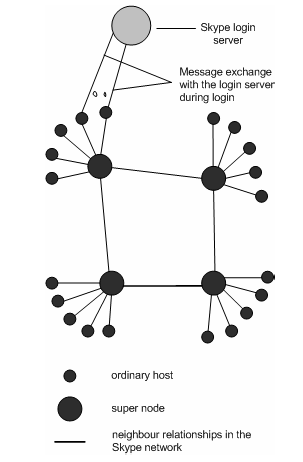
\includegraphics[width=4cm]{data/skypestructure.png}
\end{center}

Without a doubt, Skype, as a bussiness software has been reached great success in its own area --- VoIP.
The voice quality and the technique of codec is far better than other similar products.
Skype ocupied the large market share of P2P software.
However, P2P network does not provide existed solution for inevitable and potential security issues, Skype used private protocols and involved security issue, so the design and implementation were very complicated.
The management of supernodes is an onerous thing; the infomation of supernodes is stored in ordinary nodes for login and logout which is easily obtained and modified by hackers or somebody with intention, so it is more frail to suffer Sybil attack.

}

\section{Chanllenges Confronted}
{
It was because that we foucsed on the decentralized structured P2P network which was in order to avoid the design drawbacks that existed in other kinds of P2P networks, and considering with the VoD services , we should involve both the P2P overlay network and the VoD servicec based on the network we have constructed.

}
\subsection{Video File spliting ,publishing , recomposing and management}
{
  There should not be any video data centers to store and managethe video files which would send to different users to enjoy the VoD service in centralized structured P2P networks. That means we need to find an effective mechanism to handlethe actions on these video files.

Firstly, whether the video spliting is necessary or just we distribute the video files in a while block? We should consider the network service environment and anaylse the requirements which should also involve the VoD serice performance. 
In a large scaled network, a quite number of users request the same video at the same time; a great deal of connections will be established with the nodes which contain the resource files. Usually, the number of the resource nodes or seed nodes in the network is not quite many, that means less nodes will deliver the files to much more other nodes.
In this situation , the decentralized network will degrage to the semi-centralied network, these seed nodes will become the supernodes then. this is not what we expected.
As the mentioned above, we need to splite the video files into pieces and deliver the each piece to separate nodes.
Inspired from BT and eMule but not the same, we need to change the design so as to fix the request the VoD service.
And the \emph{granularity} of the spliting stream should be estimated.

Secondly, before spliting, the video stream may be encoded as many different formats, such as mp4, rmvb, wav, and so on.
So we should make the decision that whether we convert video stream from different formats to the controllable \emph{OGG}  format before delivering or just after gethering the pieces from the network and recomposing them then we convert the stream format.
Acutally, no matter when we convert the stream in the whole process, it is inevitable. The visible diffeerence is if we convert the stream after gethering data, the user impact is much more obvious. The client supported to user should pay much time to do converting and playing at the same time, which should influent the performance of VoD. However, if we just do it before delivering, the impact was just foucsed on the process of publishing.
And the efficiency we consumed in publishing will not impact user experience starkly.

Thirdly, what kind of swarming mechanism we should take. The mechanism will determine the attribute of \emph{KadPeer} project.
Usually, there are two kinds of mechanisms for data gethering -- push and pull. Both of the two are based on the Gossip algorithm. Much more effort and anaylse has been done in \cite{LargeScaleLiveMedia} and \cite{PushbasedSceduling}.

}

\subsection{Content Distribution and Search}
{
  As what we have assumed, there is no data center in the global internet, the publishing action is user spontaneous, so all of the data should be distributed in the whole system, which brings us chanllenges that it is hard to locate the chunks or segments which composed the total video files that user may request.
This part of phases depends on the mechanism we choose for swarming and diffusion.
And we also assumed the whole network is decentralized structured , so each peer will has a unique identifier. 
First connects the bootstrapping peers and selects one or several peers to construct logical links. 
Every peer maintains a group of logical neighbours and a routing table.
Peer selection is according to the routing table mentioned above.
This is also the spirit of \emph{DHT} and \emph{Overlay network}.
The key issue here is the data content distribution should match the logical routing mechanism for locating and searching.

Compared with the existed applications, just a few of them are focusing on the feature of user spontaneously publishing.
My purpose is to design and implement an easy accessing and high performancing \emph{VODFS-liked} system as an important component of the VoD application, which make peers faciliate to publishing their video data and to swarm video chunks from the other peers.

}

\subsection{Buffer / Cache}
{
As a basic function of \emph{VoD} , playback and random-index play are the most important features for \emph{VoD} applications.
To faciliate users with high quality and less response time, the application should have to decide upon the cache buffer size and cache.
}

\subsection{Stream Scheduler and metadata}
{
The scheduler keeps track of all the media content, which can be considered as a fraction of distribution and swarming mechanism.
Here, I prefer to explain the relationship between scheduler and metadata in my project.
My purpose is to design a effective method to maintain the scheduler according to the meta data which may affect the implementation of the VoD application.
An efficient and good quality matadata infrastructure for Video on demand can help in browsing and searching through the videos.
The chuncks of a specific video may attain to the peer disorderly, there should be a prepared Buffer-Map table which defines all of the chuncks splited from the whole video bulk.
The metadata could contain the Buffer-Map which is used to index the chuncks of a video and provide an absolute timing sequence of playing process which could be easily handled by the video exhibition engine.
Moreover, the metadata could be published as an item of program list which could be searched by the users who are interested in the keywords that the matadata contained.

Also there is another way to mantian the chunck order or time sequence without metadata.
There are field selections in \emph{OGG stream} with the name of \emph{bitstream serial number} and \emph{page sequence number} which define the logical bitstream identify and the page sequence. 
The sequence number increasing on each logical bitstream separetely can identify page page loss by the decoder.
However, in this situation, if we implement the scheduler just depending on the sequence number provided by the bitstream itself, the function of search should be weaken and raise the difficulty standard of decoder, especially when the bitstream contains multipule logical streams or stream groups.
This is not what we expected.
}

\subsection{GUI and Video exhibition}
{
This is the most user impact part of the \emph{VoD} application. It provides the GUI client to the users or customers and also provides control pane for item selecting, jumping forwards ,jumping backwards and other actions.
I did not pay much effort on the design of user interface, because this is not the most important thing for the current phase. It could be the future task of my project.
However, Video exhibition should be the most urgent issue of the system which determines the performance of the VoD simulation.

As for the video exhibition feature, it should contain three components --  video , audio and caption.
The key chanllenge of this issue should be the integration of the three components.
Currently, there are much many media player on the market including the opensource and non-opensource.
My project is \emph{OGG} bitstream based and current the resources of common media players are stored in local or ordered stream from the internet such as \emph{RTP} and \emph{RTSP}, that means I have to implement a codec which can distinguish the three kinds of streams with disodered chuncks and also can exhibit them to the users.
}

\section{Summary}
{
In this chapter, I have illustrated the decline of P2P traffic, the core reason is that the traffic has been hiden behind the VPN service.
I have analysed the drawbacks of centralized and semi-centralied P2P network which is inevitable because of the design.
And also I provide the chanllenges that I have confronted in the design and implementation.

}
